\documentclass[12pt,twoside]{article}
% =====================================================================
%  preambulo.tex
%  Paquetes, configuración de página y estilo para bloques de código.
%  Se carga desde main.tex con % =====================================================================
%  preambulo.tex
%  Paquetes, configuración de página y estilo para bloques de código.
%  Se carga desde main.tex con % =====================================================================
%  preambulo.tex
%  Paquetes, configuración de página y estilo para bloques de código.
%  Se carga desde main.tex con \input{preambulo}
% =====================================================================

% ---------------------------------------------------------------------
%  Codificación, idioma y fuentes
% ---------------------------------------------------------------------
\usepackage[T1]{fontenc}          % acentos y guiones correctos en español
\usepackage[utf8]{inputenc}
\usepackage{lmodern}              % versión vectorial de Computer Modern
\usepackage[spanish, provide=*]{babel}

% ---------------------------------------------------------------------
%  Geometría de página y encabezados
% ---------------------------------------------------------------------
\usepackage[a4paper, width=150mm, top=25mm, bottom=25mm, bindingoffset=6mm]{geometry}
\usepackage{fancyhdr}
\setlength{\headheight}{15.4pt}   % evita el warning de fancyhdr
\pagestyle{fancy}
\fancyhead{}
\fancyhead[LO,LE]{\leftmark}
\fancyfoot{}
\fancyfoot[CO,CE]{\thepage}
\renewcommand{\headrulewidth}{0.2pt}
\renewcommand{\footrulewidth}{0.2pt}

% ---------------------------------------------------------------------
%  Colores (antes que otros paquetes que puedan cargarlo)
% ---------------------------------------------------------------------
\usepackage[dvipsnames,table]{xcolor}

% ---------------------------------------------------------------------
%  Matemáticas y símbolos
% ---------------------------------------------------------------------
\usepackage{amsmath}
\usepackage{amssymb}
\usepackage{textcomp}
\usepackage{siunitx}

% ---------------------------------------------------------------------
%  Tablas
% ---------------------------------------------------------------------
\usepackage{array}
\usepackage{longtable}
\usepackage{multirow}
\usepackage{bigstrut}
\usepackage{booktabs}
\usepackage{tabularx}

% ---------------------------------------------------------------------
%  Figuras y páginas horizontales
% ---------------------------------------------------------------------
\usepackage{graphicx}
\usepackage{adjustbox}
\usepackage{float}
\usepackage{lscape}
\usepackage{pdflscape}

% ---------------------------------------------------------------------
%  Bibliografía (formato IEEE: citas numéricas entre corchetes)
% ---------------------------------------------------------------------
\usepackage{notoccite}
\usepackage[numbers, sort&compress]{natbib}
\usepackage[nottoc]{tocbibind}

% ---------------------------------------------------------------------
%  Código fuente: paquete listings + estilo "codigo"
% ---------------------------------------------------------------------
\usepackage{listings}

% Paleta inspirada en la imagen de referencia
\definecolor{codFondo}{HTML}{FAFAFB}      % fondo casi blanco
\definecolor{codMarco}{HTML}{D0D0D5}      % borde gris claro
\definecolor{codTexto}{HTML}{2B2B2B}      % variables e identificadores
\definecolor{codPalabra}{HTML}{5B8BC9}    % def, if, else, return...
\definecolor{codFuncion}{HTML}{4A7FC1}    % nombres de funciones (emph)
\definecolor{codNumero}{HTML}{6AA56A}     % números
\definecolor{codComentario}{HTML}{8C8C8C} % comentarios
\definecolor{codCadena}{HTML}{C1693C}     % cadenas de texto
\definecolor{codNumLinea}{HTML}{A0A0A0}   % números de línea

% Colorea los dígitos solo cuando están en código (no en comentarios ni cadenas)
\makeatletter
\newcommand{\codDigito}[1]{%
  \ifnum\lst@mode=\lst@Pmode\relax
    {\color{codNumero}#1}%
  \else
    #1%
  \fi
}
\makeatother

\lstdefinestyle{codigo}{
  language=Python,
  % --- Tipografía y colores ---
  basicstyle=\ttfamily\small\color{codTexto},
  identifierstyle=\color{codTexto},
  keywordstyle=\color{codPalabra},
  keywordstyle=[2]\color{codPalabra},
  emphstyle=\color{codFuncion},
  commentstyle=\color{codComentario},
  stringstyle=\color{codCadena},
  % --- Palabras reservadas adicionales ---
  morekeywords=[2]{True, False, None, self, nonlocal, async, await},
  % --- Marco y fondo ---
  backgroundcolor=\color{codFondo},
  frame=single,
  frameround=tttt,          % las cuatro esquinas redondeadas
  framerule=0.6pt,
  rulecolor=\color{codMarco},
  framesep=8pt,
  xleftmargin=9pt,
  xrightmargin=9pt,
  aboveskip=1em,
  belowskip=1em,
  % --- Espaciado y cortes de línea ---
  columns=fullflexible,
  keepspaces=true,
  showstringspaces=false,
  tabsize=4,
  breaklines=true,
  breakatwhitespace=true,
  postbreak=\mbox{\textcolor{codComentario}{$\hookrightarrow$}\space},
  upquote=true,
  % --- Números de línea (cambia a "left" si los quieres) ---
  numbers=none,
  numberstyle=\tiny\color{codNumLinea},
  % --- Acentos en español y coloreado de números ---
  extendedchars=true,
  literate=
    {á}{{\'a}}1 {é}{{\'e}}1 {í}{{\'i}}1 {ó}{{\'o}}1 {ú}{{\'u}}1
    {Á}{{\'A}}1 {É}{{\'E}}1 {Í}{{\'I}}1 {Ó}{{\'O}}1 {Ú}{{\'U}}1
    {ñ}{{\~n}}1 {Ñ}{{\~N}}1 {ü}{{\"u}}1 {Ü}{{\"U}}1
    {¿}{{?`}}1 {¡}{{!`}}1
    {0}{{\codDigito{0}}}1 {1}{{\codDigito{1}}}1 {2}{{\codDigito{2}}}1
    {3}{{\codDigito{3}}}1 {4}{{\codDigito{4}}}1 {5}{{\codDigito{5}}}1
    {6}{{\codDigito{6}}}1 {7}{{\codDigito{7}}}1 {8}{{\codDigito{8}}}1
    {9}{{\codDigito{9}}}1
}

% Estilo por defecto para todos los lstlisting
\lstset{style=codigo}

% Nombres en español para leyendas e índice de códigos
\renewcommand{\lstlistingname}{Código}
\renewcommand{\lstlistlistingname}{Índice de códigos}

% ---------------------------------------------------------------------
%  Enlaces (hyperref debe ir al final)
% ---------------------------------------------------------------------
\usepackage{url}
\usepackage[hidelinks]{hyperref}
% =====================================================================

% ---------------------------------------------------------------------
%  Codificación, idioma y fuentes
% ---------------------------------------------------------------------
\usepackage[T1]{fontenc}          % acentos y guiones correctos en español
\usepackage[utf8]{inputenc}
\usepackage{lmodern}              % versión vectorial de Computer Modern
\usepackage[spanish, provide=*]{babel}

% ---------------------------------------------------------------------
%  Geometría de página y encabezados
% ---------------------------------------------------------------------
\usepackage[a4paper, width=150mm, top=25mm, bottom=25mm, bindingoffset=6mm]{geometry}
\usepackage{fancyhdr}
\setlength{\headheight}{15.4pt}   % evita el warning de fancyhdr
\pagestyle{fancy}
\fancyhead{}
\fancyhead[LO,LE]{\leftmark}
\fancyfoot{}
\fancyfoot[CO,CE]{\thepage}
\renewcommand{\headrulewidth}{0.2pt}
\renewcommand{\footrulewidth}{0.2pt}

% ---------------------------------------------------------------------
%  Colores (antes que otros paquetes que puedan cargarlo)
% ---------------------------------------------------------------------
\usepackage[dvipsnames,table]{xcolor}

% ---------------------------------------------------------------------
%  Matemáticas y símbolos
% ---------------------------------------------------------------------
\usepackage{amsmath}
\usepackage{amssymb}
\usepackage{textcomp}
\usepackage{siunitx}

% ---------------------------------------------------------------------
%  Tablas
% ---------------------------------------------------------------------
\usepackage{array}
\usepackage{longtable}
\usepackage{multirow}
\usepackage{bigstrut}
\usepackage{booktabs}
\usepackage{tabularx}

% ---------------------------------------------------------------------
%  Figuras y páginas horizontales
% ---------------------------------------------------------------------
\usepackage{graphicx}
\usepackage{adjustbox}
\usepackage{float}
\usepackage{lscape}
\usepackage{pdflscape}

% ---------------------------------------------------------------------
%  Bibliografía (formato IEEE: citas numéricas entre corchetes)
% ---------------------------------------------------------------------
\usepackage{notoccite}
\usepackage[numbers, sort&compress]{natbib}
\usepackage[nottoc]{tocbibind}

% ---------------------------------------------------------------------
%  Código fuente: paquete listings + estilo "codigo"
% ---------------------------------------------------------------------
\usepackage{listings}

% Paleta inspirada en la imagen de referencia
\definecolor{codFondo}{HTML}{FAFAFB}      % fondo casi blanco
\definecolor{codMarco}{HTML}{D0D0D5}      % borde gris claro
\definecolor{codTexto}{HTML}{2B2B2B}      % variables e identificadores
\definecolor{codPalabra}{HTML}{5B8BC9}    % def, if, else, return...
\definecolor{codFuncion}{HTML}{4A7FC1}    % nombres de funciones (emph)
\definecolor{codNumero}{HTML}{6AA56A}     % números
\definecolor{codComentario}{HTML}{8C8C8C} % comentarios
\definecolor{codCadena}{HTML}{C1693C}     % cadenas de texto
\definecolor{codNumLinea}{HTML}{A0A0A0}   % números de línea

% Colorea los dígitos solo cuando están en código (no en comentarios ni cadenas)
\makeatletter
\newcommand{\codDigito}[1]{%
  \ifnum\lst@mode=\lst@Pmode\relax
    {\color{codNumero}#1}%
  \else
    #1%
  \fi
}
\makeatother

\lstdefinestyle{codigo}{
  language=Python,
  % --- Tipografía y colores ---
  basicstyle=\ttfamily\small\color{codTexto},
  identifierstyle=\color{codTexto},
  keywordstyle=\color{codPalabra},
  keywordstyle=[2]\color{codPalabra},
  emphstyle=\color{codFuncion},
  commentstyle=\color{codComentario},
  stringstyle=\color{codCadena},
  % --- Palabras reservadas adicionales ---
  morekeywords=[2]{True, False, None, self, nonlocal, async, await},
  % --- Marco y fondo ---
  backgroundcolor=\color{codFondo},
  frame=single,
  frameround=tttt,          % las cuatro esquinas redondeadas
  framerule=0.6pt,
  rulecolor=\color{codMarco},
  framesep=8pt,
  xleftmargin=9pt,
  xrightmargin=9pt,
  aboveskip=1em,
  belowskip=1em,
  % --- Espaciado y cortes de línea ---
  columns=fullflexible,
  keepspaces=true,
  showstringspaces=false,
  tabsize=4,
  breaklines=true,
  breakatwhitespace=true,
  postbreak=\mbox{\textcolor{codComentario}{$\hookrightarrow$}\space},
  upquote=true,
  % --- Números de línea (cambia a "left" si los quieres) ---
  numbers=none,
  numberstyle=\tiny\color{codNumLinea},
  % --- Acentos en español y coloreado de números ---
  extendedchars=true,
  literate=
    {á}{{\'a}}1 {é}{{\'e}}1 {í}{{\'i}}1 {ó}{{\'o}}1 {ú}{{\'u}}1
    {Á}{{\'A}}1 {É}{{\'E}}1 {Í}{{\'I}}1 {Ó}{{\'O}}1 {Ú}{{\'U}}1
    {ñ}{{\~n}}1 {Ñ}{{\~N}}1 {ü}{{\"u}}1 {Ü}{{\"U}}1
    {¿}{{?`}}1 {¡}{{!`}}1
    {0}{{\codDigito{0}}}1 {1}{{\codDigito{1}}}1 {2}{{\codDigito{2}}}1
    {3}{{\codDigito{3}}}1 {4}{{\codDigito{4}}}1 {5}{{\codDigito{5}}}1
    {6}{{\codDigito{6}}}1 {7}{{\codDigito{7}}}1 {8}{{\codDigito{8}}}1
    {9}{{\codDigito{9}}}1
}

% Estilo por defecto para todos los lstlisting
\lstset{style=codigo}

% Nombres en español para leyendas e índice de códigos
\renewcommand{\lstlistingname}{Código}
\renewcommand{\lstlistlistingname}{Índice de códigos}

% ---------------------------------------------------------------------
%  Enlaces (hyperref debe ir al final)
% ---------------------------------------------------------------------
\usepackage{url}
\usepackage[hidelinks]{hyperref}
% =====================================================================

% ---------------------------------------------------------------------
%  Codificación, idioma y fuentes
% ---------------------------------------------------------------------
\usepackage[T1]{fontenc}          % acentos y guiones correctos en español
\usepackage[utf8]{inputenc}
\usepackage{lmodern}              % versión vectorial de Computer Modern
\usepackage[spanish, provide=*]{babel}

% ---------------------------------------------------------------------
%  Geometría de página y encabezados
% ---------------------------------------------------------------------
\usepackage[a4paper, width=150mm, top=25mm, bottom=25mm, bindingoffset=6mm]{geometry}
\usepackage{fancyhdr}
\setlength{\headheight}{15.4pt}   % evita el warning de fancyhdr
\pagestyle{fancy}
\fancyhead{}
\fancyhead[LO,LE]{\leftmark}
\fancyfoot{}
\fancyfoot[CO,CE]{\thepage}
\renewcommand{\headrulewidth}{0.2pt}
\renewcommand{\footrulewidth}{0.2pt}

% ---------------------------------------------------------------------
%  Colores (antes que otros paquetes que puedan cargarlo)
% ---------------------------------------------------------------------
\usepackage[dvipsnames,table]{xcolor}

% ---------------------------------------------------------------------
%  Matemáticas y símbolos
% ---------------------------------------------------------------------
\usepackage{amsmath}
\usepackage{amssymb}
\usepackage{textcomp}
\usepackage{siunitx}

% ---------------------------------------------------------------------
%  Tablas
% ---------------------------------------------------------------------
\usepackage{array}
\usepackage{longtable}
\usepackage{multirow}
\usepackage{bigstrut}
\usepackage{booktabs}
\usepackage{tabularx}

% ---------------------------------------------------------------------
%  Figuras y páginas horizontales
% ---------------------------------------------------------------------
\usepackage{graphicx}
\usepackage{adjustbox}
\usepackage{float}
\usepackage{lscape}
\usepackage{pdflscape}

% ---------------------------------------------------------------------
%  Bibliografía (formato IEEE: citas numéricas entre corchetes)
% ---------------------------------------------------------------------
\usepackage{notoccite}
\usepackage[numbers, sort&compress]{natbib}
\usepackage[nottoc]{tocbibind}

% ---------------------------------------------------------------------
%  Código fuente: paquete listings + estilo "codigo"
% ---------------------------------------------------------------------
\usepackage{listings}

% Paleta inspirada en la imagen de referencia
\definecolor{codFondo}{HTML}{FAFAFB}      % fondo casi blanco
\definecolor{codMarco}{HTML}{D0D0D5}      % borde gris claro
\definecolor{codTexto}{HTML}{2B2B2B}      % variables e identificadores
\definecolor{codPalabra}{HTML}{5B8BC9}    % def, if, else, return...
\definecolor{codFuncion}{HTML}{4A7FC1}    % nombres de funciones (emph)
\definecolor{codNumero}{HTML}{6AA56A}     % números
\definecolor{codComentario}{HTML}{8C8C8C} % comentarios
\definecolor{codCadena}{HTML}{C1693C}     % cadenas de texto
\definecolor{codNumLinea}{HTML}{A0A0A0}   % números de línea

% Colorea los dígitos solo cuando están en código (no en comentarios ni cadenas)
\makeatletter
\newcommand{\codDigito}[1]{%
  \ifnum\lst@mode=\lst@Pmode\relax
    {\color{codNumero}#1}%
  \else
    #1%
  \fi
}
\makeatother

\lstdefinestyle{codigo}{
  language=Python,
  % --- Tipografía y colores ---
  basicstyle=\ttfamily\small\color{codTexto},
  identifierstyle=\color{codTexto},
  keywordstyle=\color{codPalabra},
  keywordstyle=[2]\color{codPalabra},
  emphstyle=\color{codFuncion},
  commentstyle=\color{codComentario},
  stringstyle=\color{codCadena},
  % --- Palabras reservadas adicionales ---
  morekeywords=[2]{True, False, None, self, nonlocal, async, await},
  % --- Marco y fondo ---
  backgroundcolor=\color{codFondo},
  frame=single,
  frameround=tttt,          % las cuatro esquinas redondeadas
  framerule=0.6pt,
  rulecolor=\color{codMarco},
  framesep=8pt,
  xleftmargin=9pt,
  xrightmargin=9pt,
  aboveskip=1em,
  belowskip=1em,
  % --- Espaciado y cortes de línea ---
  columns=fullflexible,
  keepspaces=true,
  showstringspaces=false,
  tabsize=4,
  breaklines=true,
  breakatwhitespace=true,
  postbreak=\mbox{\textcolor{codComentario}{$\hookrightarrow$}\space},
  upquote=true,
  % --- Números de línea (cambia a "left" si los quieres) ---
  numbers=none,
  numberstyle=\tiny\color{codNumLinea},
  % --- Acentos en español y coloreado de números ---
  extendedchars=true,
  literate=
    {á}{{\'a}}1 {é}{{\'e}}1 {í}{{\'i}}1 {ó}{{\'o}}1 {ú}{{\'u}}1
    {Á}{{\'A}}1 {É}{{\'E}}1 {Í}{{\'I}}1 {Ó}{{\'O}}1 {Ú}{{\'U}}1
    {ñ}{{\~n}}1 {Ñ}{{\~N}}1 {ü}{{\"u}}1 {Ü}{{\"U}}1
    {¿}{{?`}}1 {¡}{{!`}}1
    {0}{{\codDigito{0}}}1 {1}{{\codDigito{1}}}1 {2}{{\codDigito{2}}}1
    {3}{{\codDigito{3}}}1 {4}{{\codDigito{4}}}1 {5}{{\codDigito{5}}}1
    {6}{{\codDigito{6}}}1 {7}{{\codDigito{7}}}1 {8}{{\codDigito{8}}}1
    {9}{{\codDigito{9}}}1
}

% Estilo por defecto para todos los lstlisting
\lstset{style=codigo}

% Nombres en español para leyendas e índice de códigos
\renewcommand{\lstlistingname}{Código}
\renewcommand{\lstlistlistingname}{Índice de códigos}

% ---------------------------------------------------------------------
%  Enlaces (hyperref debe ir al final)
% ---------------------------------------------------------------------
\usepackage{url}
\usepackage[hidelinks]{hyperref} % paquetes, formato de página y estilo de código

\begin{document}
\sloppy
\bibliographystyle{achemso} %citation style change as necessary

\begin{titlepage}
\begin{center}
         
\includegraphics[width=15cm]{logos} %this is to have the logo
         \vspace{3cm}
         
        \Large
        \textbf{IMPLEMENTACIÓN DE ALGORITMO PSO}\\
        \vspace{0.5cm}
        \large
       Práctica 2
     
        \vspace{3cm}
     \large
        \textbf{Alcántara López Wendy Yuritzi \\Robles Guzmán Naomi Isabel  } %add any letters that should follow like B.Sc. or M.Sc. or AMRSC etc
        \vspace{0.5cm}
        \normalsize
        
        \textbf{6AV1} 
        \vspace{0.5cm}
        \large 
        
        \textbf{Profesor: }Ary Shared Rosas Carrillo
        \vfill
            
        \large
        Bioinformática \\
        24 de septiembre de 2026
            
    \end{center}

\end{titlepage}
 %title file for the front page
\tableofcontents %make table of contents (título "Índice general" provisto automáticamente por babel spanish)

%\include{Thanks-abstact} % Abstract and Acknowledgements

%edit these to suit you, add/remove as necessary. Use \include{filetitle} to add a .tex for each chapter
\pagenumbering{arabic} %necessary to start numbering pages in arabic numerals from here
\setcounter{page}{1} 

\section{Introducción}
Los problemas de optimización aparecen en prácticamente todas las áreas de la ingeniería y la ciencia, desde el ajuste de parámetros en modelos de aprendizaje automático hasta el diseño de estructuras y el control de sistemas dinámicos. Muchos de estos problemas no tienen una solución analítica sencilla: la función objetivo puede ser no lineal, no convexa, o carecer de una expresión derivable que permita aplicar métodos clásicos basados en gradiente. En estos casos, las metaheurísticas bioinspiradas ofrecen una alternativa práctica, ya que buscan soluciones aceptables sin requerir información detallada sobre la estructura del problema.
\\\\
La Optimización por Enjambre de Partículas (PSO, por sus siglas en inglés) es una de estas metaheurísticas. Fue propuesta por Kennedy y Eberhart en 1995 a partir de la observación del comportamiento colectivo de bandadas de aves y bancos de peces, donde cada individuo ajusta su trayectoria con base en su propia experiencia y en la información compartida por el grupo. Esta idea se tradujo en un algoritmo donde un conjunto de partículas explora el espacio de búsqueda, actualizando su posición y velocidad en función de su mejor resultado histórico y del mejor resultado encontrado por el enjambre.
\\\\
El comportamiento del algoritmo depende en gran medida de sus parámetros de control, en particular del peso de inercia, que regula el equilibrio entre exploración y explotación durante la búsqueda. En su formulación original, este peso permanece constante a lo largo de todas las iteraciones. Sin embargo, trabajos posteriores mostraron que variar la inercia de forma dinámica, ya sea disminuyéndola o aumentándola conforme avanza el proceso, puede mejorar la capacidad del algoritmo para converger hacia mejores soluciones.
\\\\
En esta práctica se implementa primero la versión clásica de PSO, con parámetros fijos, y después se extiende en dos pasos. Primero se hace variable únicamente el peso de inercia $w$, con una estrategia lineal decreciente y otra basada en el fitness de cada partícula. Después se hacen variables los tres coeficientes $w$, $c_1$ y $c_2$, siguiendo el esquema de coeficientes de aceleración variables en el tiempo (TVAC). El objetivo es comparar estos enfoques y analizar el efecto que tiene cada modificación sobre el comportamiento del enjambre y la calidad de las soluciones obtenidas.
\section{Marco Teórico}

\subsection{Introducción a la Computación Evolutiva y Optimización por Enjambres}

La Computación Evolutiva agrupa un conjunto de técnicas metaheurísticas de optimización inspiradas en procesos naturales, dentro de las cuales se ubican los algoritmos bio-inspirados de inteligencia colectiva o \textit{swarm intelligence}. A diferencia de los algoritmos evolutivos clásicos (como los algoritmos genéticos), que basan su búsqueda en operadores de selección, cruza y mutación aplicados sobre una población de individuos, los algoritmos de enjambre prescinden de dichos operadores genéticos y en su lugar hacen evolucionar a la población mediante la cooperación y la competencia entre sus propios integrantes~\cite{pereira_particle_2011}.

Esta familia de algoritmos toma como referencia el comportamiento colectivo observado en sistemas biológicos, como las bandadas de aves, los bancos de peces o las colonias de insectos, en los cuales ningún individuo posee información global del entorno, pero el intercambio de información local entre vecinos permite que el grupo en su conjunto localice recursos o soluciones de manera eficiente. El sociobiólogo E. O. Wilson planteó ya en 1975 que, en teoría, los miembros de un banco de peces pueden beneficiarse de los descubrimientos y la experiencia previa de todos los demás miembros durante la búsqueda de alimento, idea que sirvió de base conceptual para trasladar este principio de ``información compartida'' al ámbito de la optimización computacional~\cite{collet_stochastic_2007}.

Dentro de la inteligencia de enjambres se distinguen principalmente dos vertientes: la Optimización por Colonia de Hormigas (\textit{Ant Colony Optimization}) y la Optimización por Enjambre de Partículas (\textit{Particle Swarm Optimization}, PSO), siendo esta última el algoritmo objeto de este trabajo. Ambas comparten el principio de que una población de agentes simples, que interactúan siguiendo reglas locales, puede dar lugar a un comportamiento colectivo capaz de resolver problemas de optimización complejos que serían difíciles de abordar mediante métodos puramente individuales.

%%%%%%%%%%%%%%%%%%%%%%%%%%%%%%%%%%%%%%%%%%%%%%%%%%%%%
\subsection{Optimización por Enjambre de Partículas (PSO)}

La Optimización por Enjambre de Partículas fue propuesta originalmente por James Kennedy y Russell Eberhart en 1995, como un método para la optimización de funciones no lineales continuas. El algoritmo surgió a partir de la simulación de un modelo social simplificado, por lo que, aunque su formulación conserva la metáfora social que le dio origen, el algoritmo puede sostenerse y aplicarse de manera independiente de dicha metáfora~\cite{kennedy_particle_nodate}.

En su planteamiento inicial, Kennedy y Eberhart se apoyaron en los trabajos previos de Craig Reynolds sobre modelos de bandadas (\textit{flocking}) y observaron que, al simplificar dicho modelo eliminando las reglas relacionadas con la evasión de colisiones entre individuos, el comportamiento visual del grupo dejaba de asemejarse a una bandada y pasaba a comportarse como un enjambre; de ahí el nombre de \textit{Particle Swarm Optimization}~\cite{collet_stochastic_2007}.

En PSO, la población recibe el nombre de enjambre (\textit{swarm}) y cada individuo se denomina partícula. Cada partícula representa una posible solución candidata dentro de un espacio de búsqueda de $n$ dimensiones y se desplaza por dicho espacio ajustando su trayectoria en función de dos fuentes de información: su propia experiencia (la mejor posición que ella misma ha encontrado hasta el momento) y la experiencia del enjambre en su conjunto (la mejor posición encontrada por cualquier partícula del grupo). Ninguna partícula desaparece durante la ejecución del algoritmo; en cambio, el enjambre completo converge progresivamente hacia regiones prometedoras del espacio de búsqueda mediante un mecanismo de intercambio de información entre sus miembros~\cite{patel_fuzzy_2011}.

PSO se clasifica como un algoritmo metaheurístico, ya que realiza pocas o ninguna suposición sobre el problema que se está optimizando, lo que le permite explorar espacios de soluciones candidatas de gran tamaño y dimensionalidad. Entre sus principales ventajas se encuentran la sencillez conceptual de su implementación ---que puede programarse en pocas líneas de código---, el bajo costo computacional en términos de memoria y velocidad, y el requerir únicamente operadores matemáticos primitivos~\cite{kennedy_particle_nodate}.

A partir de su formulación original, el algoritmo ha dado lugar a numerosas variantes orientadas a mejorar su desempeño y a resolver problemas de convergencia identificados en versiones posteriores de estudio, entre las que destaca la incorporación del peso de inercia (\textit{inertia weight}) propuesto por Shi y Eberhart, así como el factor de constricción introducido por Clerc y Kennedy en 2002, ambos orientados a equilibrar la exploración y la explotación del espacio de búsqueda a lo largo de las iteraciones~\cite{freitas_particle_2020}.

%%%%%%%%%%%%%%%%%%%%%%%%%%%%%%%%%%%%%%%%%%%%%%%%%%%%%%
\subsection{Formulación matemática del algoritmo}

En PSO, cada partícula $i$ del enjambre se representa mediante un vector de posición $X_i$ y un vector de velocidad $V_i$ dentro de un espacio de búsqueda de $n$ dimensiones. En cada iteración, la posición de la partícula se actualiza sumando su velocidad actual a su posición actual~\cite{nasr_benchmarking_2020}:
\begin{equation}
\vec{X}_{id}(t+1) = \vec{X}_{id}(t) + \vec{V}_{id}(t+1)
\end{equation}
donde el subíndice $d$ denota la dimensión considerada. La velocidad, a su vez, se actualiza de acuerdo con la siguiente expresión:
\begin{equation}
\vec{V}_{id}(t+1) = w\,\vec{V}_{id}(t) + c_1 r_1 \left(P_{id} - \vec{X}_{id}(t)\right) + c_2 r_2 \left(G_d - \vec{X}_{id}(t)\right)
\end{equation}
Los elementos de esta ecuación tienen el siguiente significado:
\begin{itemize}
    \item \textbf{$w$:} peso de inercia (\textit{inertia weight}), parámetro incorporado posteriormente a la formulación original por Shi y Eberhart para controlar la influencia de la velocidad previa de la partícula sobre su velocidad actual, regulando así el balance entre exploración y explotación del espacio de búsqueda.
    \item \textbf{$P_{id}$:} mejor posición histórica encontrada por la propia partícula $i$ en la dimensión $d$ (componente cognitivo o de ``nostalgia simple'', en términos de los autores originales).
    \item \textbf{$G_d$:} mejor posición encontrada por cualquier partícula del enjambre completo en la dimensión $d$ (componente social).
    \item \textbf{$c_1$, $c_2$:} coeficientes de aceleración cognitivo y social, respectivamente, que ponderan la atracción de la partícula hacia su propio mejor histórico y hacia el mejor global del enjambre. Kennedy y Eberhart asignaron originalmente un valor de 2 a ambos coeficientes, de modo que el producto con un número aleatorio de media 0.5 diera, en promedio, un peso de 1, otorgando a la partícula probabilidades equivalentes de sobrepasar o quedarse corta respecto de su objetivo.
    \item \textbf{$r_1$, $r_2$:} números aleatorios distribuidos uniformemente en el intervalo $[0, 1]$, que introducen un componente estocástico en la búsqueda e impiden que todas las partículas converjan exactamente por la misma trayectoria.
\end{itemize}

Respecto al equilibrio entre los componentes cognitivo y social, los estudios experimentales de los autores originales mostraron que un valor de $c_1$ considerablemente mayor que $c_2$ provoca que las partículas exploren de forma errática y aislada el espacio de búsqueda, mientras que la situación inversa ---un $c_2$ mucho mayor que $c_1$--- conduce a una convergencia prematura hacia óptimos locales; los mejores resultados se obtienen generalmente cuando ambos coeficientes toman valores aproximadamente iguales~\cite{collet_stochastic_2007}.

El algoritmo se ejecuta de manera iterativa: en cada ciclo se evalúa la función objetivo (o función de aptitud) para la posición actual de cada partícula, se actualizan $P_{id}$ y $G_d$ cuando corresponde, y se recalculan velocidad y posición según las ecuaciones anteriores, repitiendo el proceso hasta alcanzar un criterio de paro, ya sea un número máximo de iteraciones o un umbral de convergencia sobre la calidad de la solución encontrada.

%%%%%%%%%%%%%%%%%%%%%%%%%%%%%%%%%%%%%%%%%%%%%%%%%%%%%%
\subsection{Parámetros del algoritmo}
\label{sec:parametros}

El desempeño de PSO depende en gran medida de la elección de sus parámetros de control. A diferencia de otros métodos de optimización, el algoritmo tiene pocos parámetros, pero pequeños cambios en su valor pueden hacer que el enjambre converja rápidamente, se estanque en un óptimo local o incluso diverja~\cite{poli2007overview, shi1998parameter}.

\begin{itemize}
    \item \textbf{Tamaño del enjambre ($N$):} número de partículas que exploran el espacio de búsqueda. Un enjambre grande cubre más regiones del espacio en cada iteración, pero aumenta el número de evaluaciones de la función objetivo. En la práctica se usan típicamente entre 20 y 50 partículas, y el algoritmo es poco sensible a este valor dentro de ese rango~\cite{poli2007overview, shi1999empirical}.

    \item \textbf{Número de iteraciones ($T$):} determina el presupuesto de cómputo y funciona como criterio de paro. En las estrategias de inercia dinámica también define la velocidad con que cambian los coeficientes, ya que estos se expresan en función de la razón $t/T$.

    \item \textbf{Peso de inercia ($w$):} escala la velocidad de la iteración anterior. Shi y Eberhart~\cite{shi1998modified} lo introdujeron para controlar el alcance de la búsqueda y encontraron que los valores entre 0.9 y 1.2 daban buenos resultados con $c_1 = c_2 = 2$. Si $w > 1$ la velocidad tiende a crecer en cada iteración y el enjambre puede divergir, mientras que un valor cercano a cero elimina la memoria del movimiento y la partícula depende solo de las atracciones hacia $P_i$ y $G$~\cite{shi1998parameter}.

    \item \textbf{Coeficientes de aceleración ($c_1$, $c_2$):} ponderan la atracción cognitiva y social. Su valor clásico es $c_1 = c_2 = 2$~\cite{kennedy1995pso}, aunque se ha demostrado que su efecto no puede analizarse por separado del de $w$, porque los tres coeficientes determinan juntos si la trayectoria de la partícula converge u oscila~\cite{clerc2002particle}.

    \item \textbf{Velocidad máxima ($V_{max}$):} límite que se aplica a cada componente de la velocidad para evitar que las partículas salgan del espacio de búsqueda. En la versión original era el único mecanismo para controlar la explosión de las velocidades. Con la incorporación de $w$ su papel se volvió secundario, y suele fijarse como una fracción del rango de cada variable~\cite{eberhart2000comparing}.
\end{itemize}

Clerc y Kennedy~\cite{clerc2002particle} analizaron la estabilidad de la trayectoria de una partícula y propusieron el factor de constricción $\chi$, que multiplica toda la ecuación de velocidad:
\begin{equation}
    \chi = \frac{2}{\left|\, 2 - \varphi - \sqrt{\varphi^2 - 4\varphi} \,\right|}, \qquad \varphi = c_1 + c_2 > 4.
    \label{eq:constriccion}
\end{equation}
Con el valor habitual $\varphi = 4.1$ se obtiene $\chi \approx 0.7298$. Esta formulación es algebraicamente equivalente a usar un peso de inercia $w = 0.7298$ y coeficientes $c_1 = c_2 = 0.7298 \cdot 2.05 \approx 1.49618$. Por esta razón estos valores se han vuelto una configuración de referencia en la literatura~\cite{eberhart2000comparing, poli2007overview}, y son los que se usan en la implementación con coeficientes fijos de esta práctica.

%%%%%%%%%%%%%%%%%%%%%%%%%%%%%%%%%%%%%%%%%%%%%%%%%%%%%%
\subsection{El dilema exploración vs. explotación}
\label{sec:exploracion}

Todo algoritmo de búsqueda metaheurística debe equilibrar dos objetivos opuestos. La \textit{exploración} consiste en visitar regiones nuevas del espacio de búsqueda para no pasar por alto zonas prometedoras. La \textit{explotación} consiste en refinar la búsqueda alrededor de las mejores soluciones encontradas para mejorar su precisión~\cite{crepinsek2013exploration}. Un algoritmo que explora demasiado se comporta como una búsqueda aleatoria y tarda en converger. Uno que explota demasiado converge rápido, pero puede quedar atrapado en el primer óptimo local que encuentre, un fenómeno conocido como convergencia prematura~\cite{crepinsek2013exploration, zhan2009adaptive}.

En PSO, cada término de la ecuación de velocidad contribuye de forma distinta a este equilibrio:
\begin{itemize}
    \item El término de inercia $w\,V_i$ mantiene la dirección de movimiento de la partícula. Un valor grande de $w$ le permite recorrer distancias largas y favorece la exploración global, mientras que un valor pequeño concentra la búsqueda en una región local~\cite{shi1998modified, shi1998parameter}.
    \item El componente cognitivo $c_1 r_1 (P_i - X_i)$ atrae a cada partícula hacia su propia mejor posición. Como cada partícula tiene un $P_i$ distinto, este término mantiene la diversidad del enjambre y favorece la exploración~\cite{ratnaweera2004self}.
    \item El componente social $c_2 r_2 (G - X_i)$ atrae a todas las partículas hacia el mismo punto. Este término acelera la convergencia y favorece la explotación, pero también reduce la diversidad del enjambre~\cite{ratnaweera2004self}.
\end{itemize}

El equilibrio adecuado no es el mismo durante toda la ejecución. Al inicio conviene explorar, porque el enjambre todavía no tiene información sobre la ubicación del óptimo. Al final conviene explotar, porque el enjambre ya identificó una región prometedora y lo que importa es refinar la solución~\cite{shi1999empirical, zhan2009adaptive}. Esto es especialmente importante en funciones multimodales como Rastrigin, cuya gran cantidad de óptimos locales castiga tanto la convergencia prematura como la falta de convergencia. Un conjunto de coeficientes fijos representa un único compromiso entre ambos objetivos para toda la ejecución, lo que motiva el uso de coeficientes que cambian con el tiempo.

%%%%%%%%%%%%%%%%%%%%%%%%%%%%%%%%%%%%%%%%%%%%%%%%%%%%%%
\subsection{PSO con inercia dinámica}
\label{sec:inercia_dinamica}

En la variante con inercia dinámica, $w$ deja de ser constante y se ajusta durante la ejecución para pasar de un comportamiento exploratorio a uno explotador. Bansal et al.~\cite{bansal2011inertia} compararon quince estrategias propuestas en la literatura, que pueden agruparse en tres familias:

\begin{itemize}
    \item \textbf{Estrategias dependientes del tiempo.} $w$ cambia en función de la iteración, sin usar información del enjambre. La más conocida es la inercia lineal decreciente (LDIW, por sus siglas en inglés) de Shi y Eberhart~\cite{shi1999empirical}:
    \begin{equation}
        w(t) = w_{max} - (w_{max} - w_{min})\,\frac{t}{T},
        \label{eq:ldiw}
    \end{equation}
    con los valores recomendados $w_{max} = 0.9$ y $w_{min} = 0.4$. Existen también versiones no lineales, en las que $w$ decrece siguiendo una potencia de $t/T$~\cite{chatterjee2006nonlinear}.

    \item \textbf{Estrategias aleatorias.} $w$ se muestrea en cada iteración, por ejemplo $w = 0.5 + \mathrm{rand}()/2$, lo que produce un valor medio de 0.75. Eberhart y Shi~\cite{eberhart2001tracking} la propusieron para problemas cuyo óptimo cambia con el tiempo, donde no tiene sentido reducir $w$ de forma monótona.

    \item \textbf{Estrategias adaptativas.} $w$ se calcula a partir del estado del enjambre, por ejemplo la calidad de la solución de cada partícula, la tasa de partículas que mejoraron su mejor posición o la dispersión del enjambre~\cite{nickabadi2011novel, zhan2009adaptive}. A diferencia de las anteriores, estas estrategias pueden asignar un valor de $w$ distinto a cada partícula. La estrategia basada en fitness de esta práctica pertenece a esta familia.
\end{itemize}

La misma idea puede extenderse a los coeficientes de aceleración. Ratnaweera et al.~\cite{ratnaweera2004self} propusieron los coeficientes de aceleración variables en el tiempo (TVAC), en los que $c_1$ disminuye y $c_2$ aumenta linealmente durante la ejecución:
\begin{equation}
    c_1(t) = c_{1i} + (c_{1f} - c_{1i})\,\frac{t}{T}, \qquad
    c_2(t) = c_{2i} + (c_{2f} - c_{2i})\,\frac{t}{T}.
    \label{eq:tvac}
\end{equation}
Con $c_{1i} = 2.5$, $c_{1f} = 0.5$, $c_{2i} = 0.5$ y $c_{2f} = 2.5$, al inicio domina el componente cognitivo y las partículas se mueven de forma independiente. Al final domina el componente social y el enjambre se concentra alrededor del mejor global. Combinado con la inercia de la ecuación~\eqref{eq:ldiw}, este esquema obtuvo mejores resultados que el PSO con inercia lineal y coeficientes fijos en la mayoría de las funciones de prueba evaluadas por sus autores~\cite{ratnaweera2004self}.
\section{Desarrollo de la práctica}
\subsection{Variante 1: PSO con parámetros fijos (clásico)}
En la variante clásica el coeficiente de inercia $w$ tiene el mismo valor durante toda la ejecución. Este coeficiente determina qué tanto conserva cada partícula su velocidad anterior en la actualización
\begin{equation}
v_i^{t+1} = w\,v_i^{t} + c_1 r_1 \left(p_i - x_i^{t}\right) + c_2 r_2 \left(g - x_i^{t}\right),
\label{eq:velocidad}
\end{equation}
donde $p_i$ es la mejor posición encontrada por la partícula $i$ y $g$ es la mejor posición del enjambre. Un $w$ alto favorece la exploración porque las partículas recorren distancias grandes sin cambiar mucho de dirección. Un $w$ bajo favorece la explotación porque el movimiento depende casi por completo de las atracciones hacia $p_i$ y $g$.

\subsubsection{Interfaz común para las estrategias de \texorpdfstring{$w$}{w}}

Para comparar las estrategias sin duplicar el algoritmo, cada una se implementó como una función que recibe la iteración actual \texttt{t}, el número total de iteraciones \texttt{T}, el vector con el fitness de las partículas y el generador de números aleatorios \texttt{rng}. La función devuelve un escalar cuando todas las partículas comparten el mismo $w$, o un vector con un valor por partícula. Cada estrategia se construye con una función externa que fija sus parámetros y devuelve la función interna \texttt{w}. Con esta forma, el $w$ constante de la variante 1 también se puede expresar como una estrategia:

\begin{lstlisting}[emph={w_constante, w}, caption={Estrategia de $w$ constante (variante 1)}]
def w_constante(valor):
    # Enfoque 1: w fijo durante todas las iteraciones.
    def w(t, T, fitness, rng):
        return valor
    return w
\end{lstlisting}

\subsection{Variante 2: PSO con inercia dinámica}
\label{subsec:inercia_dinamica}

 En la inercia dinámica, $w$ cambia durante la ejecución para ajustar ese equilibrio. En esta práctica se implementaron dos estrategias: una que reduce $w$ linealmente con las iteraciones y otra que asigna a cada partícula un $w$ calculado a partir de su fitness.



\subsubsection{Inercia lineal decreciente}

La primera estrategia empieza con un valor alto de $w$ y lo reduce en cada iteración hasta un valor mínimo:
\begin{equation}
w(t) = w_{max} - \frac{(w_{max} - w_{min})\,t}{T},
\label{eq:w_lineal}
\end{equation}
donde $t$ es la iteración actual y $T$ el número total de iteraciones. Se usaron $w_{max} = 0.9$ y $w_{min} = 0.4$, los mismos valores del cuaderno original. Al inicio las partículas se mueven con mucha inercia y exploran el espacio de búsqueda; conforme avanza la ejecución, la inercia disminuye y el enjambre se concentra alrededor de las mejores soluciones encontradas. Como el ciclo recorre $t = 0, 1, \dots, T-1$, el último valor aplicado es $0.9 - 0.5 \cdot 999/1000 \approx 0.4005$.

\begin{lstlisting}[emph={w_lineal, w}, caption={Estrategia de $w$ lineal decreciente}]
def w_lineal(wmax, wmin):
    # Enfoque 2: w = wmax - (wmax - wmin) * t / T
    def w(t, T, fitness, rng):
        return wmax - (wmax - wmin) * t / T
    return w
\end{lstlisting}

En esta estrategia $w$ depende solo del número de iteración, por lo que todas las partículas usan el mismo valor en una misma iteración y la función devuelve un escalar.

\subsubsection{Inercia basada en el fitness}

La segunda estrategia calcula un $w$ distinto para cada partícula en cada iteración:
\begin{equation}
w_i = \frac{1.1 \cdot \text{rand}()}{f(x_i)},
\label{eq:w_fitness}
\end{equation}
donde $f(x_i)$ es el fitness de la posición actual de la partícula $i$ y $\text{rand}()$ es un número aleatorio uniforme en $[0, 1)$ generado de forma independiente para cada partícula. Como el problema es de minimización, una partícula con menor $f(x_i)$ recibe en promedio un $w$ más grande y conserva más de su velocidad, mientras que las partículas con mal fitness pierden inercia y quedan dominadas por la atracción hacia $p_i$ y $g$. El factor aleatorio evita que dos partículas con el mismo fitness reciban siempre el mismo valor.

\begin{lstlisting}[emph={w_fitness, w}, caption={Función de peso por partícula}]
def w_fitness(usar_error=False, f_optimo=F_OPTIMO, epsilon=1e-12):
    # Enfoque 3: w_i = 1.1 * rand() / f(x_i), un valor por partícula
    def w(t, T, fitness, rng):
        f = fitness - f_optimo if usar_error else fitness
        return 1.1 * rng.random(fitness.shape) / np.maximum(f, epsilon)
    return w
\end{lstlisting}

El resultado de la ecuación~\eqref{eq:w_fitness} depende de la escala de la función objetivo. La función F5 del CEC 2017 incluye un desplazamiento de 500 en su valor, así que $f(x_i) \geq 500$ en todo el dominio y $w_i$ nunca supera $1.1/500 = 0.0022$. Para estudiar este efecto se implementaron dos versiones controladas por el parámetro \texttt{usar\_error}:

\begin{itemize}
\item Con \texttt{usar\_error=False} se aplica la ecuación tal como está definida, usando el valor de $f(x_i)$ que devuelve el benchmark.
\item Con \texttt{usar\_error=True} el denominador es el error $f(x_i) - f^*$, con $f^* = 500$. De esta forma se elimina el desplazamiento de la función y $w_i$ puede tomar valores mayores. Cuando una partícula se acerca al óptimo el error tiende a cero y $w_i$ crece sin límite, por lo que el denominador se acota inferiormente con \texttt{epsilon} para evitar una división entre cero.
\end{itemize}

\subsubsection{Integración en el algoritmo}

La función \texttt{ejecutar\_pso} del cuaderno original calculaba $w$ con la ecuación~\eqref{eq:w_lineal} dentro del ciclo. En la nueva versión recibe la estrategia como parámetro \texttt{estrategia\_w} y la invoca en cada iteración con el fitness de las posiciones actuales. El fragmento siguiente muestra la parte del ciclo que cambió:

\begin{lstlisting}[emph={estrategia_w, w}, caption={Cálculo de $w$ y actualización de velocidad dentro de \texttt{ejecutar\_pso}}]
for it in range(num_iterations):
    r1 = rng.uniform(0, 1, size=(size, dimension))
    r2 = rng.uniform(0, 1, size=(size, dimension))

    w = np.asarray(estrategia_w(it, num_iterations, fitness, rng), dtype=float)
    historial_w[it] = w.mean()
    if w.ndim == 1:              # un w por particula
        w = w[:, None]

    velocity = (w * velocity +
                c1 * r1 * (personal_best_positions - position) +
                c2 * r2 * (global_best_position - position))

    if limitar:
        velocity = np.clip(velocity, -vmax, vmax)
        position = np.clip(position + velocity, low, high)
    else:
        position = position + velocity
\end{lstlisting}

El resultado de la estrategia se convierte a un arreglo de NumPy. Si es un escalar (estrategias constante y lineal), se multiplica directamente por la matriz de velocidades de tamaño $N \times D$. Si es un vector de $N$ elementos (estrategia basada en fitness), se reordena como una columna de tamaño $N \times 1$ con \texttt{w[:, None]}, de modo que el \emph{broadcasting} de NumPy multiplique toda la fila de velocidades de la partícula $i$ por su propio $w_i$. En cada iteración también se guarda el promedio de $w$ en \texttt{historial\_w} para graficar su evolución.

Además, se agregó un límite a la velocidad, $v_{max} = 0.2\,(x_{max} - x_{min}) = 40$, y las posiciones se recortan al espacio de búsqueda $[-100, 100]^D$. Con $c_1 = c_2 = 1.5$, las configuraciones con $w$ pequeño, como la basada en fitness, producen oscilaciones cada vez más amplias y las partículas salen del dominio. El límite se puede desactivar con \texttt{limitar=False}.

Por último, todas las configuraciones evaluadas se reúnen en un diccionario que asocia cada nombre con su enfoque y su estrategia. El experimento recorre este diccionario para cada dimensión y ejecuta 30 corridas por configuración:

\begin{lstlisting}[emph={w_constante, w_lineal, w_fitness}, caption={Configuraciones de $w$ evaluadas}]
CONFIGURACIONES = {
    "Constante w=0.4":    ("Constante", w_constante(0.4)),
    "Constante w=0.6":    ("Constante", w_constante(0.6)),
    "Constante w=0.7298": ("Constante", w_constante(0.7298)),
    "Constante w=0.9":    ("Constante", w_constante(0.9)),
    "Lineal 0.9->0.4":    ("Lineal decreciente", w_lineal(0.9, 0.4)),
    "Fitness 1.1r/f(x)":  ("Basado en fitness", w_fitness(usar_error=False)),
    "Fitness 1.1r/error": ("Basado en fitness", w_fitness(usar_error=True)),
}
\end{lstlisting}

La ejecución $k$ de cada configuración usa la semilla $2017 + 1000\,D + k$, la misma para todas las estrategias de $w$. Así, en una misma dimensión, todas las configuraciones parten de la misma población inicial y las diferencias en el desempeño se pueden atribuir a la estrategia de inercia. El desempeño de cada estrategia se analiza en la Sección~\ref{sec:resultados}.

\section{Resultados}
\label{sec:resultados}

En esta sección se presentan los resultados de PSO sobre la función F5 (Shifted and Rotated Rastrigin) del benchmark CEC 2017 en 10, 20 y 30 dimensiones. Cada configuración del coeficiente de inercia $w$ se ejecutó 30 veces con 50 partículas y 1000 iteraciones. La ejecución $k$ de cada configuración partió de la misma población inicial, de modo que las diferencias entre configuraciones se deben a la estrategia de $w$ y no a la inicialización. La métrica reportada es el error $f(x_{best}) - f^*$, donde $f^* = 500$ es el valor óptimo de F5. Ninguna ejecución alcanzó el óptimo global; el error más bajo registrado fue de 4.97, obtenido con $w$ lineal decreciente en $D=10$.

\subsection{Error final por configuración}

La Tabla~\ref{tab:pso_rastrigin} resume la media y la desviación estándar del error final. La mejor configuración de cada dimensión aparece en negritas. El símbolo entre paréntesis indica el resultado de la prueba de Wilcoxon pareada contra la mejor configuración, con corrección de Holm y $\alpha = 0.05$: (+) significa que la mejor configuración es significativamente superior y (=) que la diferencia no es significativa.

\begin{table}[H]
\centering
\caption{Error $f(x_{best})-f^*$ de PSO en F5 (Rastrigin) (media $\pm$ desviación estándar, 30 ejecuciones).}
\label{tab:pso_rastrigin}
\resizebox{\textwidth}{!}{%
\begin{tabular}{lccc}
\toprule
Configuración de $w$ & $D=10$ & $D=20$ & $D=30$ \\
\midrule
Constante $w=0.4$ & 29.442 $\pm$ 13.060 (+) & 72.037 $\pm$ 19.543 (+) & 185.764 $\pm$ 48.687 (+) \\
Constante $w=0.6$ & 25.764 $\pm$ 8.035 (+) & 64.029 $\pm$ 18.045 (+) & 139.393 $\pm$ 41.407 (+) \\
Constante $w=0.7298$ & 16.804 $\pm$ 5.990 (=) & 55.078 $\pm$ 20.177 (+) & 123.156 $\pm$ 33.203 (+) \\
Constante $w=0.9$ & 26.465 $\pm$ 6.849 (+) & 91.607 $\pm$ 16.288 (+) & 222.272 $\pm$ 21.899 (+) \\
Lineal $0.9\to0.4$ & \textbf{14.538 $\pm$ 5.690} & \textbf{37.764 $\pm$ 13.615} & \textbf{82.609 $\pm$ 29.148} \\
Fitness $1.1r/f(x)$ & 39.460 $\pm$ 12.969 (+) & 101.298 $\pm$ 23.609 (+) & 251.794 $\pm$ 40.230 (+) \\
Fitness $1.1r/\text{error}$ & 41.274 $\pm$ 12.024 (+) & 104.239 $\pm$ 22.745 (+) & 248.884 $\pm$ 38.504 (+) \\
\bottomrule
\end{tabular}%
}
\end{table}

El $w$ lineal decreciente obtuvo el menor error medio en las tres dimensiones: 14.54 en $D=10$, 37.76 en $D=20$ y 82.61 en $D=30$. La segunda posición correspondió siempre al $w$ constante de 0.7298. En $D=10$ la diferencia entre ambas no fue significativa ($p = 0.088$), pero en $D=20$ y $D=30$ sí lo fue, y la distancia entre ellas creció con la dimensión. En $D=10$ el error de $w=0.7298$ es 16\,\% mayor que el de la estrategia lineal, mientras que en $D=20$ y $D=30$ es 46\,\% y 49\,\% mayor, respectivamente.

El enfoque basado en fitness tuvo el peor desempeño en todas las dimensiones. Sus dos variantes, con $f(x)$ y con el error $f(x)-f^*$ en el denominador, dieron resultados casi idénticos (39.46 frente a 41.27 en $D=10$ y 251.79 frente a 248.88 en $D=30$). En $D=30$ su error medio triplica el de la estrategia lineal.

La Figura~\ref{fig:barras} muestra los mismos datos en forma gráfica. La desviación estándar aumenta con la dimensión en todas las configuraciones. En $D=30$ la más baja corresponde a $w=0.9$ (21.90), aunque su media (222.27) es de las más altas.

\begin{figure}[H]
\centering
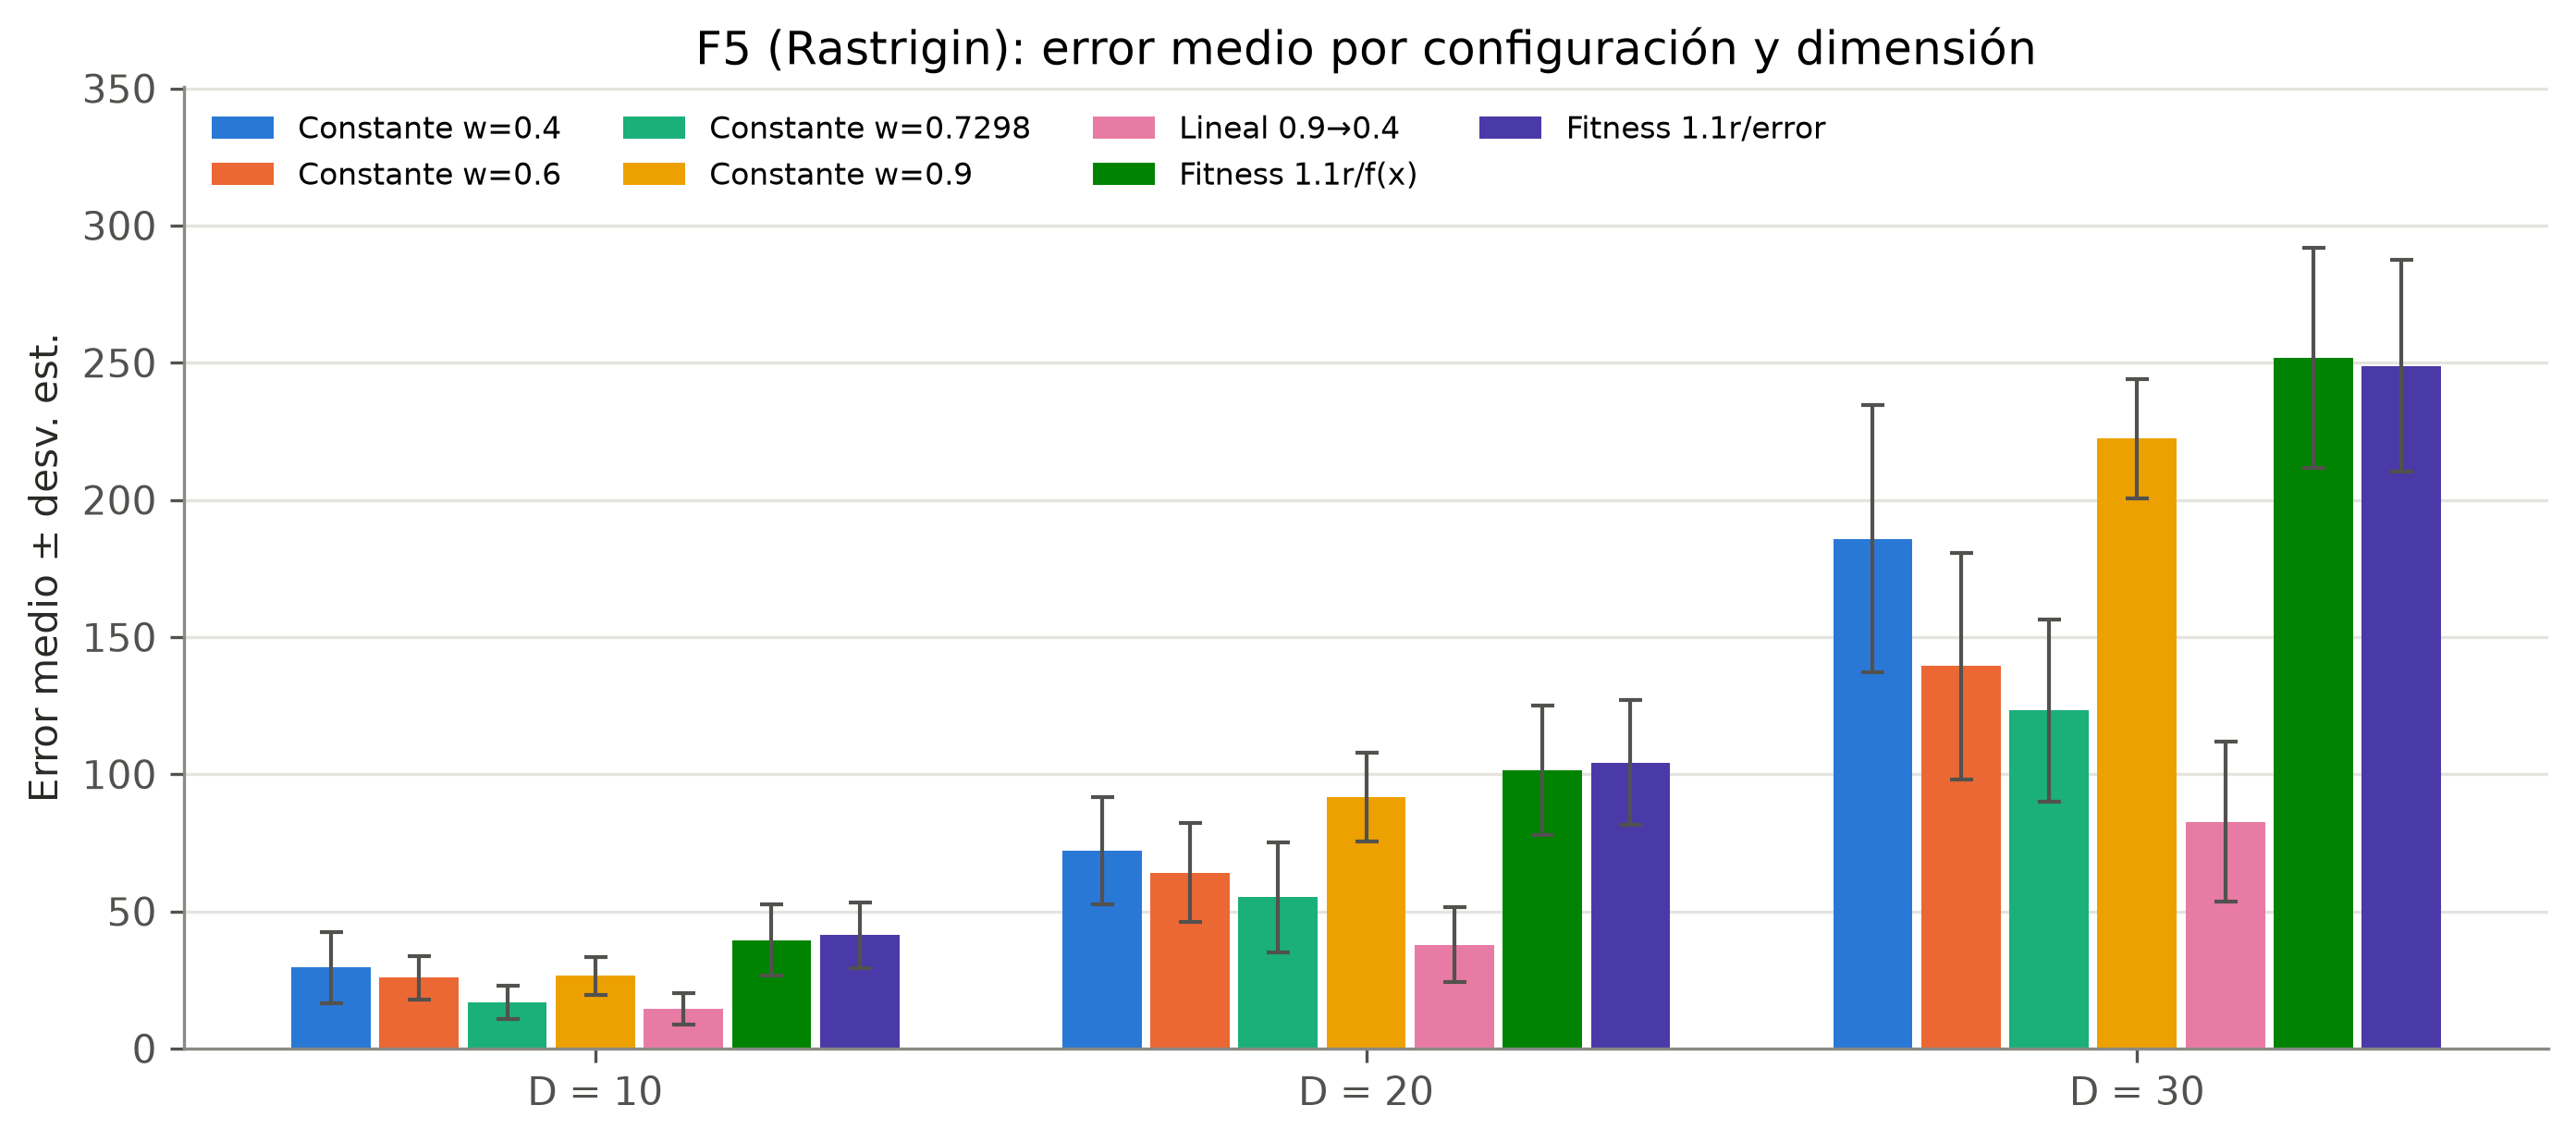
\includegraphics[width=\textwidth]{figuras/barras_media_desviacion.png}
\caption{Error medio $\pm$ desviación estándar de cada configuración de $w$ por dimensión.}
\label{fig:barras}
\end{figure}

\subsection{Distribución del error}

La Figura~\ref{fig:boxplots} muestra la distribución del error final de las 30 ejecuciones. En las tres dimensiones la caja de la estrategia lineal es la más baja, y en $D=20$ y $D=30$ su mediana (34.00 y 83.08) queda por debajo del primer cuartil de todas las demás configuraciones. En $D=30$ su tercer cuartil prácticamente coincide con el primer cuartil de $w=0.7298$.

Las dos variantes del enfoque basado en fitness tienen cajas similares entre sí y separadas del resto. En $D=10$ son además las de mayor dispersión, con errores entre 15 y 72. El $w$ constante de 0.4 también presenta una dispersión alta en las tres dimensiones y tiene la desviación estándar más grande de los valores constantes (13.06 en $D=10$ y 48.69 en $D=30$). Esto indica que su resultado depende mucho de la población inicial. Con $w=0.9$ ocurre lo contrario en $D=30$: la caja es estrecha pero está en un nivel de error alto, es decir, el algoritmo falla de manera consistente.

\begin{figure}[H]
\centering
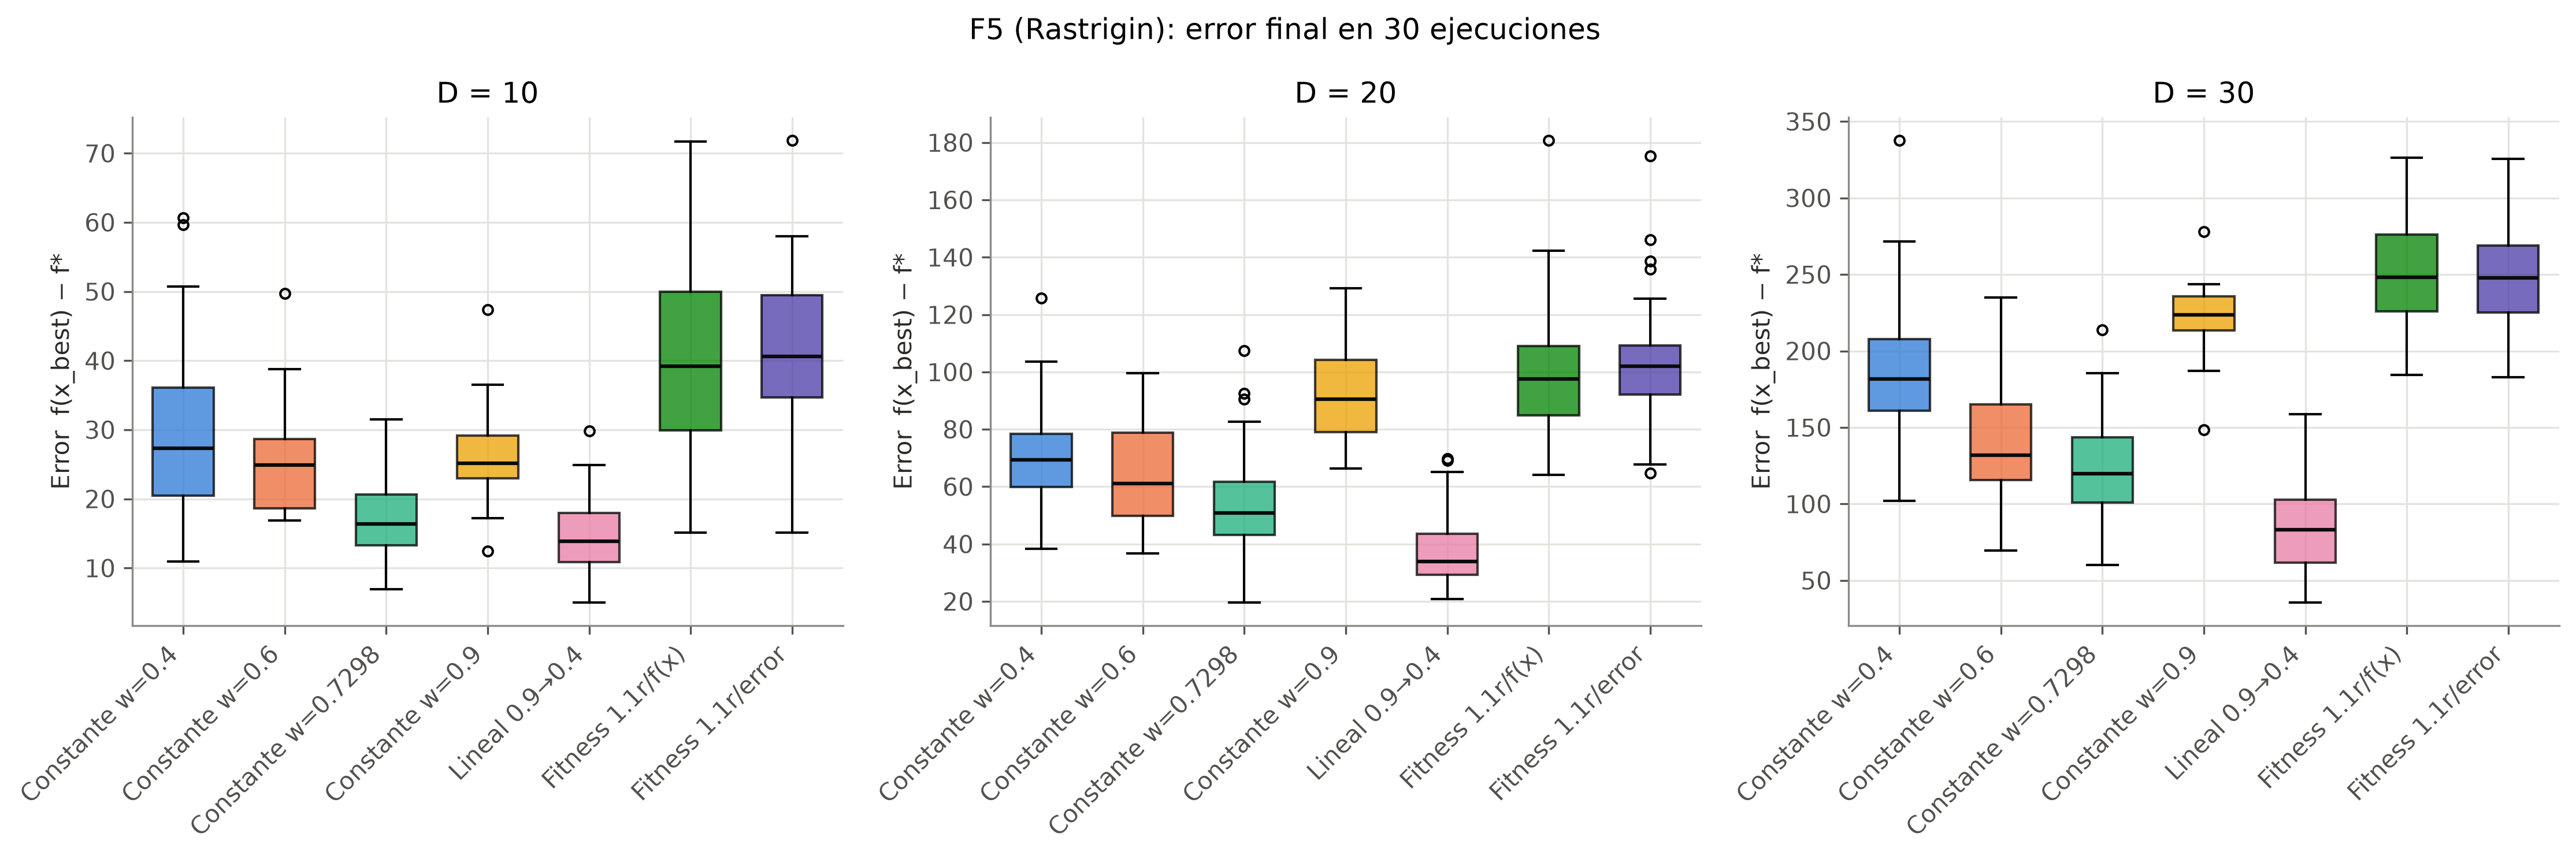
\includegraphics[width=\textwidth]{figuras/boxplots_error_final.png}
\caption{Distribución del error final en 30 ejecuciones para $D = 10$, 20 y 30.}
\label{fig:boxplots}
\end{figure}

\subsection{Sensibilidad al valor de \texorpdfstring{$w$}{w} y escalabilidad}

La gráfica izquierda de la Figura~\ref{fig:sensibilidad} muestra el error medio en función del valor de $w$ constante. En las tres dimensiones la relación tiene forma de U, con el mínimo en $w=0.7298$: valores menores provocan convergencia prematura y valores mayores impiden la convergencia. La forma se acentúa al aumentar la dimensión. En $D=10$ el error medio varía entre 16.80 y 29.44 según el valor de $w$, y en $D=30$ entre 123.16 y 222.27. Las líneas punteadas marcan el error de la estrategia lineal, que queda por debajo de todos los valores constantes probados en cada dimensión.

La gráfica derecha muestra cómo crece el error medio con la dimensión. Todas las configuraciones empeoran al pasar de 10 a 30 variables, y el crecimiento es más pronunciado entre $D=20$ y $D=30$ que entre $D=10$ y $D=20$. El orden de las configuraciones se mantiene casi igual en las tres dimensiones. La única excepción es $w=0.9$, que en $D=10$ tiene un error similar al de $w=0.6$ (26.46 frente a 25.76) y en $D=30$ es el peor de los valores constantes. La estrategia lineal pasa de 14.54 a 82.61, y es la configuración con menor error en todas las dimensiones.

\begin{figure}[H]
\centering
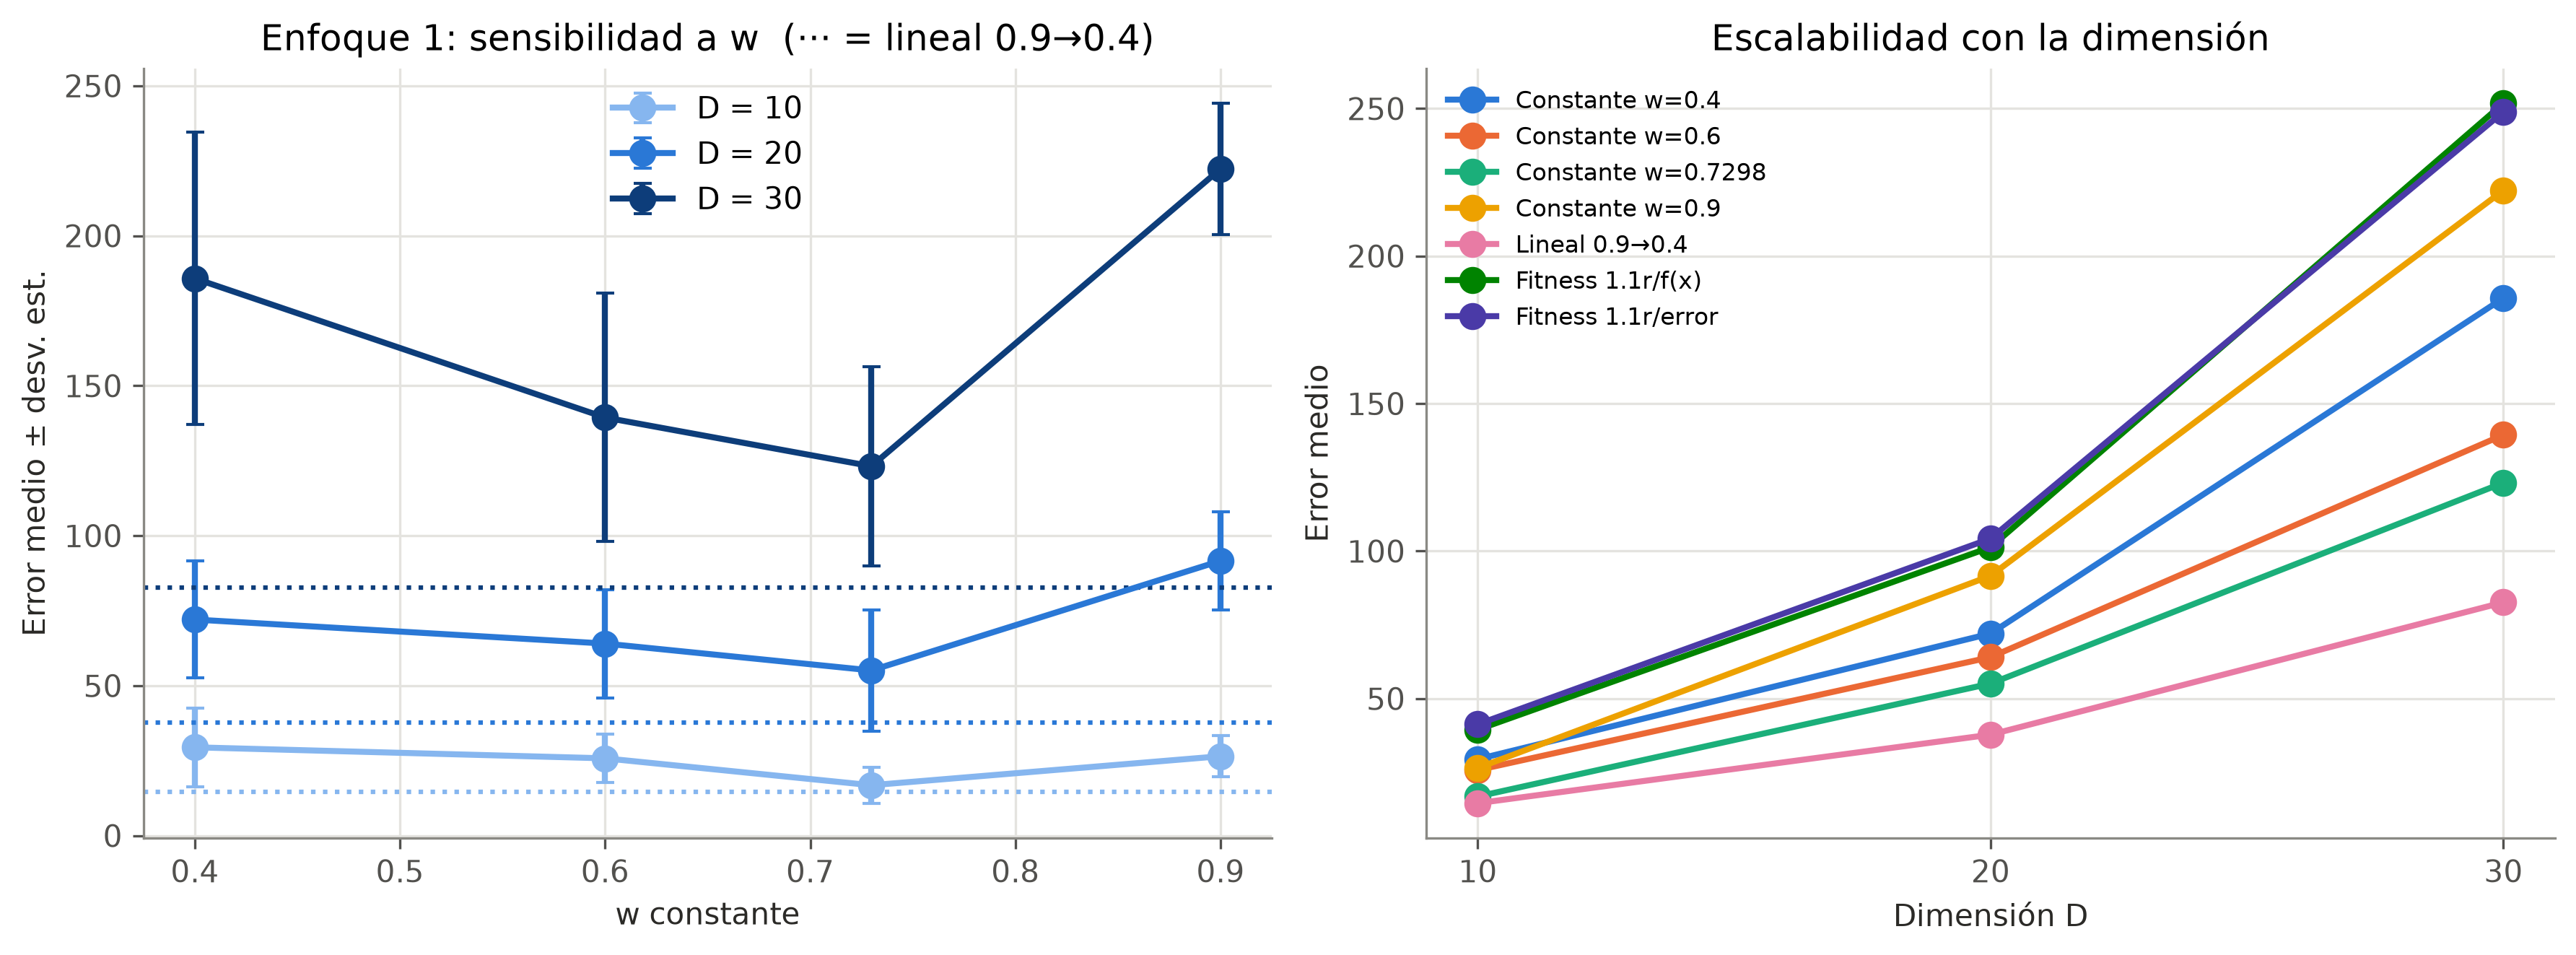
\includegraphics[width=\textwidth]{figuras/sensibilidad_y_escalabilidad.png}
\caption{Izquierda: error medio en función de $w$ constante (las líneas punteadas corresponden a la estrategia lineal $0.9\to0.4$). Derecha: error medio en función de la dimensión.}
\label{fig:sensibilidad}
\end{figure}

\section{Resultados: coeficientes fijos frente a dinámicos}
\label{sec:resultados_dinamicos}

En esta sección se comparan dos implementaciones de PSO sobre la función F5 (Shifted and Rotated Rastrigin) del benchmark CEC 2017 en 10, 20 y 30 dimensiones. A diferencia de la Sección~\ref{sec:resultados}, en la que solo cambiaba el coeficiente de inercia $w$ y se mantenía $c_1 = c_2 = 1.5$, aquí cambian los tres coeficientes $w$, $c_1$ y $c_2$. La primera implementación usa valores fijos durante toda la ejecución y la segunda los modifica en cada iteración (Tabla~\ref{tab:coeficientes}).

\begin{table}[H]
\centering
\caption{Coeficientes de las dos implementaciones de PSO.}
\label{tab:coeficientes}
\begin{tabular}{lccc}
\toprule
Implementación & $w$ & $c_1$ (cognitivo) & $c_2$ (social) \\
\midrule
PSO fijo & $0.7298$ & $1.49618$ & $1.49618$ \\
PSO dinámico & $0.9 \to 0.4$ & $2.5 \to 0.5$ & $0.5 \to 2.5$ \\
\bottomrule
\end{tabular}
\end{table}

Los valores fijos son los propuestos por Clerc y Kennedy~\cite{clerc2002particle}. En la implementación dinámica los tres coeficientes varían linealmente con la iteración $t$, siguiendo el esquema de coeficientes de aceleración variables en el tiempo (TVAC) de Ratnaweera et al.~\cite{ratnaweera2004self}:
\begin{align}
w(t)   &= w_{max} - (w_{max}-w_{min})\,\frac{t}{T}, \label{eq:tvac_w}\\
c_1(t) &= c_{1i} + (c_{1f}-c_{1i})\,\frac{t}{T}, \label{eq:tvac_c1}\\
c_2(t) &= c_{2i} + (c_{2f}-c_{2i})\,\frac{t}{T}, \label{eq:tvac_c2}
\end{align}
donde $T = 1000$ es el número total de iteraciones. Al inicio domina el componente cognitivo, que favorece la exploración, y al final domina el social, que favorece la explotación alrededor del mejor global.

Cada implementación se ejecutó 30 veces por dimensión con 50 partículas y 1000 iteraciones. Se usaron las mismas semillas que en la Sección~\ref{sec:resultados}, de modo que la ejecución $k$ de ambas implementaciones partió de la misma población inicial. La métrica reportada es el error $f(x_{best}) - f^*$, con $f^* = 500$.

\subsection{Mejor solución, media y desviación estándar}

La Tabla~\ref{tab:fijo_dinamico} presenta, para cada dimensión, la mejor solución encontrada en las 30 ejecuciones, junto con la media y la desviación estándar del error final. El mejor valor de cada dimensión aparece en negritas.

\begin{table}[H]
\centering
\caption{Resultados de PSO con coeficientes fijos y dinámicos en F5 (Rastrigin), 30 ejecuciones.}
\label{tab:fijo_dinamico}
\small
\setlength{\tabcolsep}{4pt}
\begin{tabular}{llcccc}
\toprule
$D$ & Implementación & Mejor $f(x)$ & Mejor error & Media $\pm$ desv. est. & Peor error \\
\midrule
\multirow{2}{*}{10} & PSO fijo & 505.970 & 5.970 & 17.824 $\pm$ 6.720 & 33.415 \\
 & PSO dinámico & \textbf{503.980} & \textbf{3.980} & \textbf{8.884 $\pm$ 3.485} & \textbf{16.914} \\
\midrule
\multirow{2}{*}{20} & PSO fijo & 527.980 & 27.980 & 53.493 $\pm$ 17.778 & 99.493 \\
 & PSO dinámico & \textbf{511.940} & \textbf{11.940} & \textbf{24.343 $\pm$ 8.852} & \textbf{47.758} \\
\midrule
\multirow{2}{*}{30} & PSO fijo & 578.857 & 78.857 & 123.676 $\pm$ 28.868 & 217.894 \\
 & PSO dinámico & \textbf{541.902} & \textbf{41.902} & \textbf{68.677 $\pm$ 17.727} & \textbf{108.084} \\
\bottomrule
\end{tabular}
\end{table}

La implementación dinámica obtuvo mejores resultados en todas las medidas y en las tres dimensiones. Su error medio es aproximadamente la mitad del de la implementación fija: 8.88 frente a 17.82 en $D=10$, 24.34 frente a 53.49 en $D=20$ y 68.68 frente a 123.68 en $D=30$. Su desviación estándar también es menor (3.49, 8.85 y 17.73, frente a 6.72, 17.78 y 28.87), por lo que el resultado depende menos de la población inicial. Incluso la peor ejecución de la versión dinámica en $D=20$ y $D=30$ (47.76 y 108.08) queda por debajo del error medio de la versión fija.

La Figura~\ref{fig:fijo_dinamico} resume ambas implementaciones. A la izquierda se muestra el valor de cada coeficiente a lo largo de la ejecución y a la derecha el error final medio con su desviación estándar.

\begin{figure}[H]
\centering
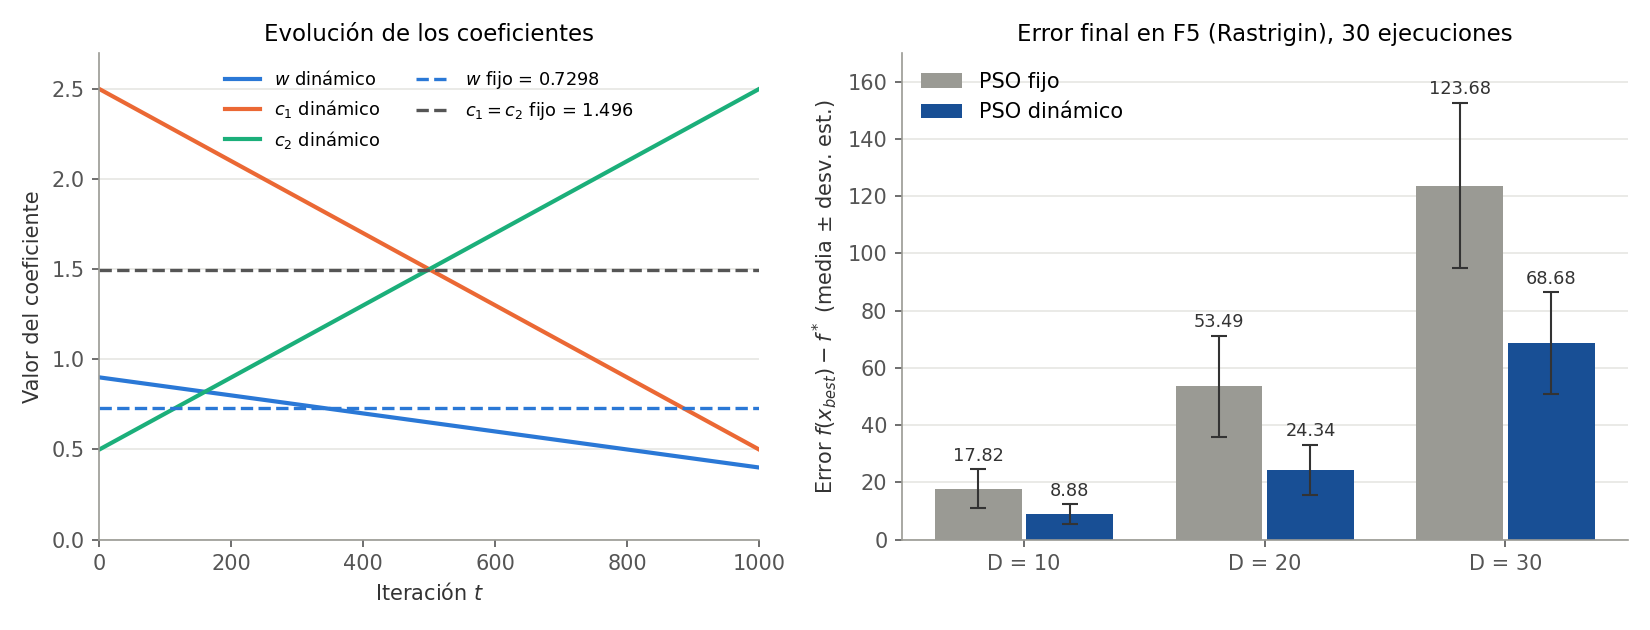
\includegraphics[width=\textwidth]{fijo_vs_dinamico.png}
\caption{Izquierda: valor de $w$, $c_1$ y $c_2$ por iteración (líneas continuas: implementación dinámica; líneas punteadas: implementación fija, donde $c_1$ y $c_2$ coinciden). Derecha: error final medio $\pm$ desviación estándar en 30 ejecuciones para $D = 10$, 20 y 30.}
\label{fig:fijo_dinamico}
\end{figure}

Ninguna ejecución alcanzó el óptimo global. La mejor solución, con $f(x) = 503.98$, se obtuvo con coeficientes dinámicos en $D=10$. Este error de 3.98 es menor que el mínimo registrado en la Sección~\ref{sec:resultados} (4.97, con $w$ lineal y $c_1 = c_2 = 1.5$).

\subsection{Convergencia}

La evolución del error del mejor global durante la ejecución, medida como la mediana de las 30 ejecuciones, explica la diferencia entre ambas implementaciones.


Con coeficientes fijos el error baja rápidamente y después se estanca. La mediana alcanza el 99\,\% de su mejora total alrededor de la iteración 143 en $D=20$ y 186 en $D=30$, y a partir de ahí la curva es prácticamente plana. En $D=20$, por ejemplo, el error mediano es 49.5 tanto en la iteración 200 como en la 1000. El enjambre converge de forma prematura a un mínimo local de Rastrigin.

Con coeficientes dinámicos, las primeras iteraciones son más lentas. En la iteración 200 el error mediano es 27.2 en $D=10$, 110.9 en $D=20$ y 230.7 en $D=30$, mayor que el de la versión fija en las tres dimensiones (19.9, 49.5 y 122.9). En esta etapa $w$ y $c_1$ son altos y $c_2$ es bajo, así que cada partícula explora cerca de su propia trayectoria y la atracción hacia el mejor global es débil. Conforme $c_2$ aumenta y $w$ disminuye, el error baja de forma pronunciada y la curva cruza a la de la versión fija cerca de la iteración 256 en $D=10$, 301 en $D=20$ y 376 en $D=30$. El cruce ocurre más tarde al aumentar la dimensión. La versión dinámica sigue mejorando hasta la iteración 372, 392 y 456, respectivamente, antes de estabilizarse.

\subsection{Pruebas estadísticas}

Como las ejecuciones de ambas implementaciones comparten semilla, se aplicó la prueba de rangos con signo de Wilcoxon para muestras pareadas. Se eligió una prueba no paramétrica porque la prueba de Shapiro--Wilk rechazó la normalidad del error en $D=20$ para ambas implementaciones y en $D=30$ para la versión fija ($\alpha = 0.05$).

\begin{table}[H]
\centering
\caption{Prueba de Wilcoxon pareada entre PSO fijo y PSO dinámico.}
\label{tab:wilcoxon_fijo_dinamico}
\small
\begin{tabular}{lccc}
\toprule
 & $D=10$ & $D=20$ & $D=30$ \\
\midrule
Mediana del error (fijo) & 16.42 & 49.53 & 117.90 \\
Mediana del error (dinámico) & \textbf{8.89} & \textbf{22.88} & \textbf{65.67} \\
Ejecuciones en que gana el dinámico & 27 / 30 & 29 / 30 & 29 / 30 \\
Valor $p$ & $1.80\times10^{-5}$ & $5.59\times10^{-9}$ & $3.73\times10^{-9}$ \\
\bottomrule
\end{tabular}
\end{table}

La diferencia a favor de la implementación dinámica es significativa en las tres dimensiones ($p < 0.001$). Partiendo de la misma población inicial, la versión dinámica terminó con menor error en 27 de las 30 ejecuciones en $D=10$ y en 29 de 30 en $D=20$ y $D=30$.

\subsection{Comparación con los resultados de la Sección~\ref{sec:resultados}}

Como se usaron las mismas semillas, los resultados también pueden compararse de forma pareada con las configuraciones de la Sección~\ref{sec:resultados}. La implementación fija no difiere significativamente de $w = 0.7298$ con $c_1 = c_2 = 1.5$ ($p = 0.349$, 0.584 y 0.855 en $D = 10$, 20 y 30), lo cual es esperable porque sus coeficientes son casi iguales.

La implementación dinámica mejora a la estrategia de $w$ lineal $0.9\to0.4$ con $c_1 = c_2 = 1.5$, que había sido la mejor configuración. El error medio pasa de 14.54 a 8.88 en $D=10$, de 37.76 a 24.34 en $D=20$ y de 82.61 a 68.68 en $D=30$. La diferencia es significativa en $D=10$ y $D=20$ ($p = 3.45\times10^{-5}$ en ambos casos), pero no en $D=30$ ($p = 0.058$), donde la versión dinámica ganó en 21 de las 30 ejecuciones. Como ambas estrategias reducen $w$ de la misma forma, esta mejora se debe a la variación de $c_1$ y $c_2$: dar más peso al componente cognitivo al inicio y al social al final ayuda a evitar la convergencia prematura en Rastrigin.
\section{Conclusiones}
 
En esta práctica se implementó PSO en su versión clásica y se extendió con distintos esquemas de coeficientes dinámicos. Todas las configuraciones se evaluaron sobre la función F5 (Rastrigin) del CEC 2017 en 10, 20 y 30 dimensiones, con 30 ejecuciones por configuración y las mismas semillas, lo que permitió compararlas de forma pareada.
 
Cuando solo se modificó el peso de inercia, la estrategia lineal decreciente ($0.9 \rightarrow 0.4$) obtuvo el menor error medio en las tres dimensiones. Con $w$ constante el error forma una U con el mínimo cerca de $w = 0.7298$: los valores bajos provocan convergencia prematura y los altos impiden converger. La estrategia basada en fitness tuvo el peor desempeño, aun después de eliminar el desplazamiento de la función.
 
Hacer variables también $c_1$ y $c_2$ (TVAC) dio los mejores resultados de toda la práctica. Frente a los coeficientes fijos, redujo el error medio aproximadamente a la mitad y también redujo su desviación estándar en las tres dimensiones, con diferencias significativas en todos los casos ($p < 0.001$). Las curvas de convergencia explican esta diferencia. Con coeficientes fijos el enjambre se estanca antes de la iteración 200, mientras que con coeficientes dinámicos avanza más lento al inicio pero sigue mejorando hasta pasadas las 350 iteraciones. Frente a la estrategia de $w$ lineal con $c_1 = c_2 = 1.5$, la mejora fue significativa en $D = 10$ y $D = 20$ pero no en $D = 30$. Como ambas reducen $w$ de la misma forma, esta ganancia se atribuye a dar más peso al componente cognitivo al inicio y al social al final.
 
En todas las configuraciones el error creció con la dimensión y ninguna ejecución alcanzó el óptimo global, lo que refleja la dificultad de Rastrigin por su gran cantidad de óptimos locales. El mejor resultado fue un error de 3.98 en $D = 10$, obtenido con coeficientes dinámicos.


\bibliography{fuentes}

%remember to either sync with Mendeley or Zotero or upload a .bib file exported from those cite using \cite{CitationTagXXXX} there will be a list it's ok
\end{document}